\colorlet{chaptergrey}{red!60!yellow!30!}
%\renewcommand*\sectfont{\color{orange}}

\chapter[Kinematic misalignment in MaNGA]{Kinematic misalignment in MaNGA}
\label{ch:kin_mis}
\vspace{-5.25in}
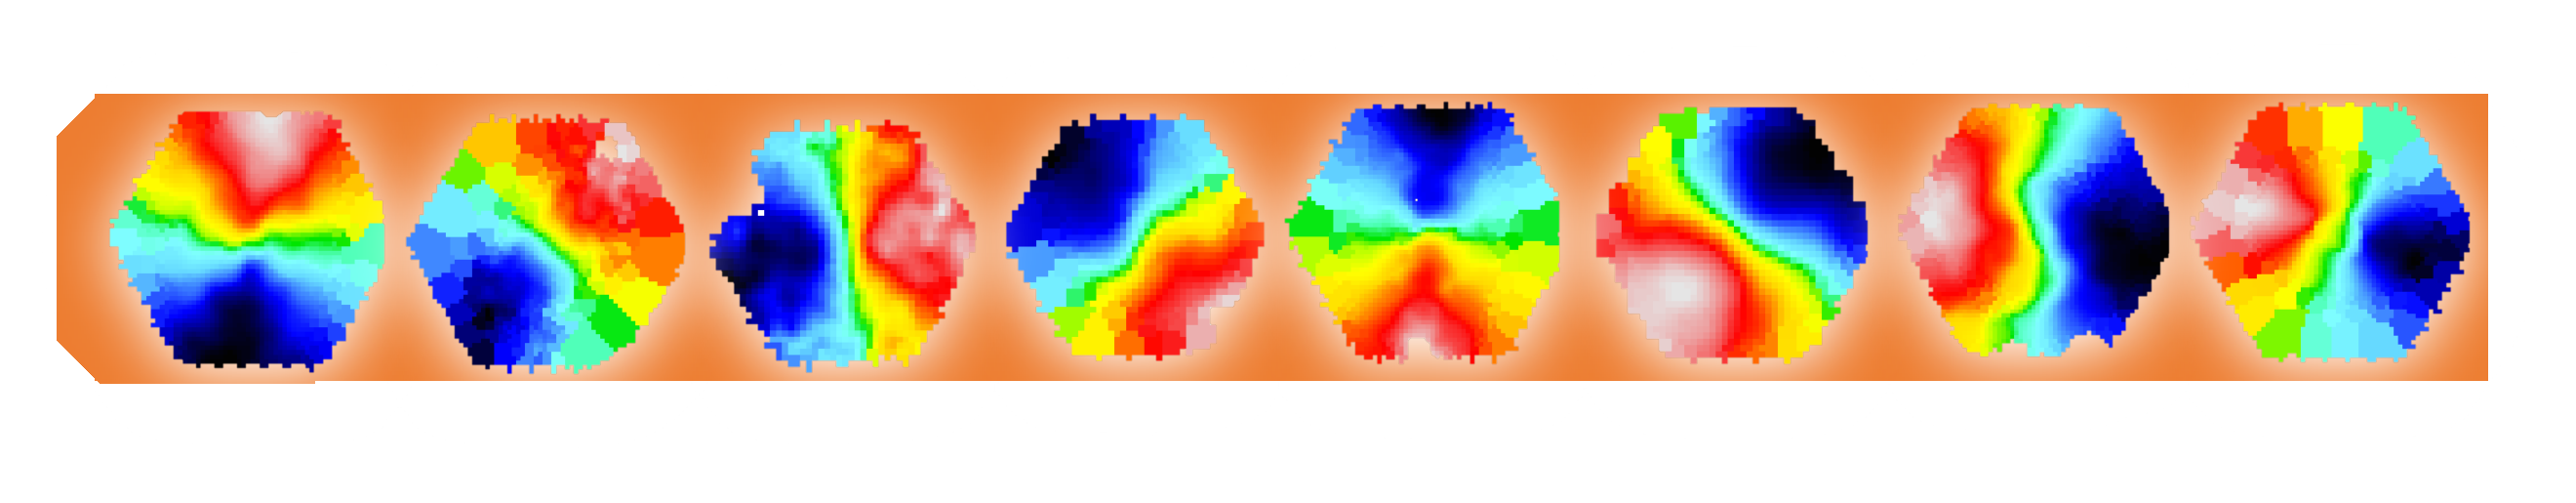
\includegraphics[height=1.39in]{thesis/latex/misalignment_MaNGA/kin_mis_chapter_heading.pdf}
\vspace{3in}

\epigraph{This chapter is partially based on Duckworth, Tojeiro, Kraljic, Sgr\'o, Wild, Weijmans, Lacerna and Drory, in MNRAS, 448, Issue 1, 2019 and Duckworth, Tojeiro and Kraljic, in MNRAS 492, Issue 2, 2020. Here, we introduce kinematic misalignment and investigate the relationship of kinematically misaligned galaxies with morphology, angular momentum and gas content in observations.} 

\section{Introduction}
Developments in spectrographs have led to the advent of integral field spectroscopy (IFS) which provides spatially resolved spectra for galaxies. Unlike single-fibre galaxy surveys such as SDSS which only obtain spectra from the central $\sim 3 ''$ of a target galaxy, IFS observations enable spatially resolved spectral measurements up-to several effective radii (\re) across the faces of nearby galaxies. From these spectra, we can simultaneously extract kinematics of stars and gas, while obtaining absorption line strengths which provide radial gradients of gas phase metallicity and stellar population age.

In kinematics, establishing work in the field has been the Spectrographic Areal Unit for Research on Optical Nebulae \citep[SAURON;][]{sauron} and ATLAS\textsuperscript{3D} \citep{atlas3d} surveys, which have focused on early type galaxies (ETGs) in the local Universe. IFS has enabled kinematic classification through a proxy for angular momentum based on the stellar kinematics up to one effective radius ($\mathrm{R_e}$). Termed $\mathrm{\lambda_{Re}}$, the measure enabled the clear distinction between slow and fast rotating ETGs \citep{emsellem2007, emsellem2011}. While there is still debate over whether 1$\mathrm{R_{e}}$ is large enough to fully encapsulate the complete kinematic morphology of a galaxy \citep{foster2013, arnold2014}, it has opened the door for understanding the relationship between optical morphology and angular momentum. 

IFS observations are costly, and such detailed information has often come at the cost of total galaxies observed. For example, in the last 10 years ATLAS\textsuperscript{3D} and CALIFA \citep{califa} observed 260 and 667 galaxies respectively with various selection criteria. IFS surveys for $\sim$1000 of galaxies across all optical morphologies are now a reality. For example, the Sydney-AAO  Multi-object  Integral  field  spectrograph  survey \citep[][]{croom2012, bryant2015} has mapped $\sim$3400 galaxies upto $z\sim0.12$ across a variety of environments. Even larger is the Mapping Nearby Galaxies at Apache Point \citep[MaNGA;][]{bundy2015, blanton2017} survey which will map $\sim$10000 galaxies in the local Universe ($z=0-0.15$). By design MaNGA will create a sample of near flat number density distribution across absolute $i$-band magnitude and stellar mass.

%Studies in more recent IFS surveys and simulations have demonstrated the close interlink between stellar angular momentum, stellar mass and morphology suggesting that late types and early type fast rotators form a continuous sequence rather than from fundamentally different formation pathways \citep[][]{cortese2016, lagos2017, graham2018}. Remarkably, despite the highly non-linear processes involved, current cosmological surveys predict that the stellar angular momentum in rotationally supported galaxies at $z=0$ is still conserved from that of the dark matter halo \citep[e.g.][]{genel2015}. 

While the stellar continuum is often considered for studies of angular momentum, optical IFS observations also provide kinematic information of the ionized gas in the galaxy. In the basic picture of TTT, stars form from the collapsing gas leading to the expectation that they inherit its dynamics and hence galaxies have coherent rotation between their stars and gas. Unsurprisingly galaxy evolution is complex and galaxies seldom form in isolation, resulting in a significant proportion of galaxies with decoupled rotation between their stars and ionized gas. 

An offset between the rotation of stars and ionized gas has been motivated to be of external origin \citep[see][]{sarzi2006,davis2011a}. The ability of a given galaxy to accrete cold gas determines its continued ability to form stars and hence dictate where it falls amongst the Hubble sequence. Accreted gas, however, has many origins (such as filamentary `cold mode' accretion from the cosmic web, mergers or additionally cooling flows from a shocked hot halo) however is converted into stars within typical depletion timescales of order gigayears \citep{davis2016}. 
For material stripped in mergers or for shocked gas accreting through cooling flows, a natural consideration is that the accretion may not be necessarily aligned with the angular momentum of the benefiting galaxy \citep[e.g.][]{davis2011, lagos2015}. Misalignment can be considered to be a transient property as torques from the stellar component continually act to realign the gas component which can only be opposed by sustained misaligned accretion \citep[][]{vdvoort2015, davis2016}. 

Understanding the origin and nature of galaxies with decoupled star-gas rotation (kinematic misalignment - used interchangeably) has been the focus for several recent works. \citet{davis2011a} found that $\sim 36$\% of ETGs exhibit misalignment between their star and gas rotation (i.e. difference of at least 30$^{\circ}$ between rotational axes) within the volume-limited sample of ATLAS\textsuperscript{3D} \citep{atlas3d}. This fraction increases when considering field ETGs, giving a first suggestion at an environmental dependence. For late types, \citet{chen2016} first investigated star forming galaxies with counter-rotating stars and gas (i.e. difference of at least 150$^{\circ}$ between rotational axes), a far rarer occurrence ($\sim$2\%), finding a clear boost in star formation in central regions. This suggests that the processes leading to significant misalignment are also inherent in cancelling angular momentum, enabling increased gas in-flows to nuclear regions. \citet{jin2016} extended this discussion to find that for a sample of 66 misaligned galaxies, the misalignment fraction ($> 30^{\circ}$) is dependent on properties such as specific star formation rate, stellar mass and local environment, again determining that misaligned galaxies are more isolated. 

Despite this, kinematic misalignment appears to be correlated with mergers and interactions. In CALIFA, \citet[][]{barrera2015} investigated a range of interacting galaxies (i.e. at different stages of a merger) in comparison to a non-interacting control. They demonstrate that interacting galaxies of all stages demonstrate both more significant misalignment between stars and gas represented in global position angles, but also that position angles are more likely to deviate as a function of radius for any given component. This is corroborated by \citet{li_decoupling2019} who investigated the relationship between kinematic misalignment in MaNGA and deeper photometry in the Dark Energy Spectroscopic Instrument (DESI) Legacy Imaging Surveys \citep{dey2019}. They find that up-to 40\% of misaligned galaxies in MaNGA can be attributed to ongoing or recent mergers/interactions, underlining the importance of external processes. 

This likely represents a lower limit on the importance of interactions due to the typical timescales of misalignment. \citet{davis2016} utilise a toy model to propose that misaligned gas could relax gradually over time-scales of 1-5 Gyr. A faster time-scale of relaxation would require merger rates of $\approx 5$ Gyr\textsuperscript{-1} and hence is disfavoured. The interplay between the strength and persistence of the gas in-flow and the re-aligning torque of the stellar component dictates the exact time-scale of misalignment for an individual galaxy. The strength of a galaxy's stellar torque scales as a function of radius, with the central component of a galaxy re-aligning on a quicker time-scale than the outer regions. The persistence of misalignment has also been considered in numerical simulations. \citet{vdvoort2015} consider the evolution of a misaligned gas disc formed from a merger which removes most of the original disc. During re-accretion of the cold gas, the misaligned disc persists for approximately 2 Gyr before the gas-star rotation angle falls below 20$^{\circ}$. The sustainment of this misalignment is due to continued gas accretion for approximately 1.5 Gyr before its rate falls and the gas can realign with the stellar component on approximately six dynamical time-scales. 

In this Chapter, we introduce the methodology of defining kinematic misalignment in the context of the MaNGA survey. We then investigate the relationship of kinematic misalignment with optical morphology, angular momentum and gas content in MaNGA observations. In \S\ref{sec:manga_intro} we introduce the MaNGA survey and associated data output (\S\ref{sec:vel_fields_intro}), before describing the methodology in defining kinematic misalignment in \S\ref{sec:kin_mis}. \S\ref{sec:data_obs} gives a description of the additional data catalogues used in this work and \S\ref{sec:results_obs} describes the observational properties of misaligned galaxies, before summarising in \S\ref{sec:summary_manga}.

\section{MaNGA} \label{sec:manga_intro}
Set to complete in 2020, the MaNGA survey is designed to investigate the internal structure of $\sim$10000 galaxies in the nearby Universe. By design, the complete sample is unbiased towards morphology, inclination and colour and provides a near flat distribution in stellar mass. 

MaNGA is one of three programs in the fourth generation of the Sloan Digital Sky Survey (SDSS-IV) which enables detailed kinematics through integral field unit (IFU) spectroscopy. MaNGA uses the SDSS 2.5 metre telescope in spectroscopic mode \citep{gunn2006} with the two dual-channel BOSS spectrographs \citep{smee2013} and the MaNGA IFUs \citep{drory2015}. MaNGA provides spatial resolution on kpc scales (2'' diameter fibres) while covering 3600-10300$\mathrm{\mathring{A}}$ in wavelength with a resolving power that varies from R$\sim$1400 at 4000$\mathrm{\mathring{A}}$ to R$\sim$2600 at 9000$\mathrm{\mathring{A}}$. 

MaNGA observations use SDSS style plates, where bundles of optical fibres are plugged into the plate corresponding to the position of the target galaxy in the observational field. A dithered pattern is employed for each target field (plate), which simultaneously observes galaxies through 17 fibre-bundles of 5 distinct sizes. Any incomplete data release of MaNGA should therefore be unbiased with respect to IFU sizes and hence a reasonable representation of the final sample scheduled to be complete in 2020.

The majority of observations contribute to one of the three main subsets: the Primary sample, the Secondary sample and the Colour-Enhanced supplement. All sub-samples observe galaxies to a minimum of $\sim 1.5$ effective radii ($\mathrm{R_{e}}$) with the Secondary sample increasing this minimum to $\sim 2.5 \mathrm{R_{e}}$. The Colour-Enhanced supplement fills in gaps of the colour-magnitude diagram leading to an approximately flat distribution of stellar mass. A full description of the MaNGA observing strategy is given in \citet{law2015obs,yan2016obs}. The raw observations are processed by the MaNGA Data Reduction Pipeline (DRP) as described in \citet{law2016drp, yan2016spec}. The fibre flux and inverse variance is extracted from each exposure, which are then wavelength calibrated, flat-fielded and sky subtracted.

MaNGA releases data periodically in the form of MaNGA Product Launches (MPL), both increasing the number of observed galaxies and updating the data processing. In the following chapters we use data from MPL-6 and MPL-8 referring to the sixth and eighth Product Launches.
% Include a figure showing the distribution of NSA, MaNGA targets, MPL-6 and MPL-8.
% Also include figure of bundle sizes?
 
\section{Velocity fields} \label{sec:vel_fields_intro}
The MaNGA Data Analysis Pipeline \citep[DAP][]{westfall2019,belfiore2019} provides science-ready processed data for MaNGA observations. Some example outputs include; spaxel-by-spaxel coordinate information based on the isophotal ellipticities from the NASA-Sloan Atlas, S/N measurements, binned spectra, stellar kinematics and stellar-continuum models, emission-line properties and models, and spectral-index measurements. Kinematics are easily accessible as 2D maps which we use for stellar and gas velocity fields in the following analysis. A complete discussion can be found in \citet{westfall2019,belfiore2019}, however we will summarise the key points concerning stellar and gas velocity fields here.

The DAP extracts stellar kinematics using the Penalised Pixel-Fitting (pPXF) method \citep{cappellari2004,cappellari2017}. The DAP fits the stellar continuum of each spaxel to extract the line of sight velocity dispersion and then fits the absorption-line spectra from a set of 49 clusters of stellar spectra from the MILES stellar library \citep{sanchez2006,falcon2011}. Before extraction of the mean stellar velocity, the spectra are spatially Voronoi binned to $g$-band \textit{S/N} $\sim$ 10, excluding any individual spectrum with a $g$-band \textit{S/N} < 1 \citep{cappellari2003}. This approach is geared towards stellar kinematics as the spatial binning is applied to the continuum \textit{S/N}, however, we note that unbinned and Voronoi binned velocity maps produce similar results. 

Ionized gas kinematics are extracted by the DAP through fitting a Gaussian to the H$\alpha$-6564 emission line, relative to the input redshift for the galaxy. This velocity is representative for all ionized gas, since the parameters for each Gaussian fit to each emission line are tied during the fitting process. These velocities are also binned spatially by the Voronoi bins of the stellar continuum. 

\section{Kinematic misalignment} \label{sec:kin_mis}
We estimate the two dimensional global position angle (PA) of the stellar and H$\alpha$ gas velocity fields using the \texttt{FIT\_KINEMATIC\_PA} routine outlined in Appendix C of \citet{krajnovic2006}. By default this finds the angle corresponding to the bisecting line which has greatest velocity change along it (i.e. the angle of peak rotational velocity). We choose this angle to be found from sampling at 180 equally spaced steps. This is measured counter-clockwise from the north axis, however, it does not discriminate between the blueshifted and redshifted side since it is only defined up to 180$^{\circ}$. As a result, velocity fields with a difference of 180$^{\circ}$ PA would appear to be aligned. To solve this we identify the direction of rotation and re-assign a consistent PA: defined as the axis of rotation approximately 90$^{\circ}$ clockwise from the blueshifted side. This angle now spans 360$^{\circ}$ allowing an automatic detection of misaligned gas and stellar components. The offset angle between kinematic components is defined as: 
\begin{equation} \label{eq:delPA}
\mathrm{\Delta PA = |PA_{stellar} - PA_{H\alpha}|. }
\end{equation}
We define galaxies with $\Delta$PA > 30$^{\circ}$ to be significantly kinematically misaligned. An example of an aligned and a misaligned galaxy is shown in Figure \ref{fig:cutout_wIFU}. 

\begin{figure*}
    \centering
	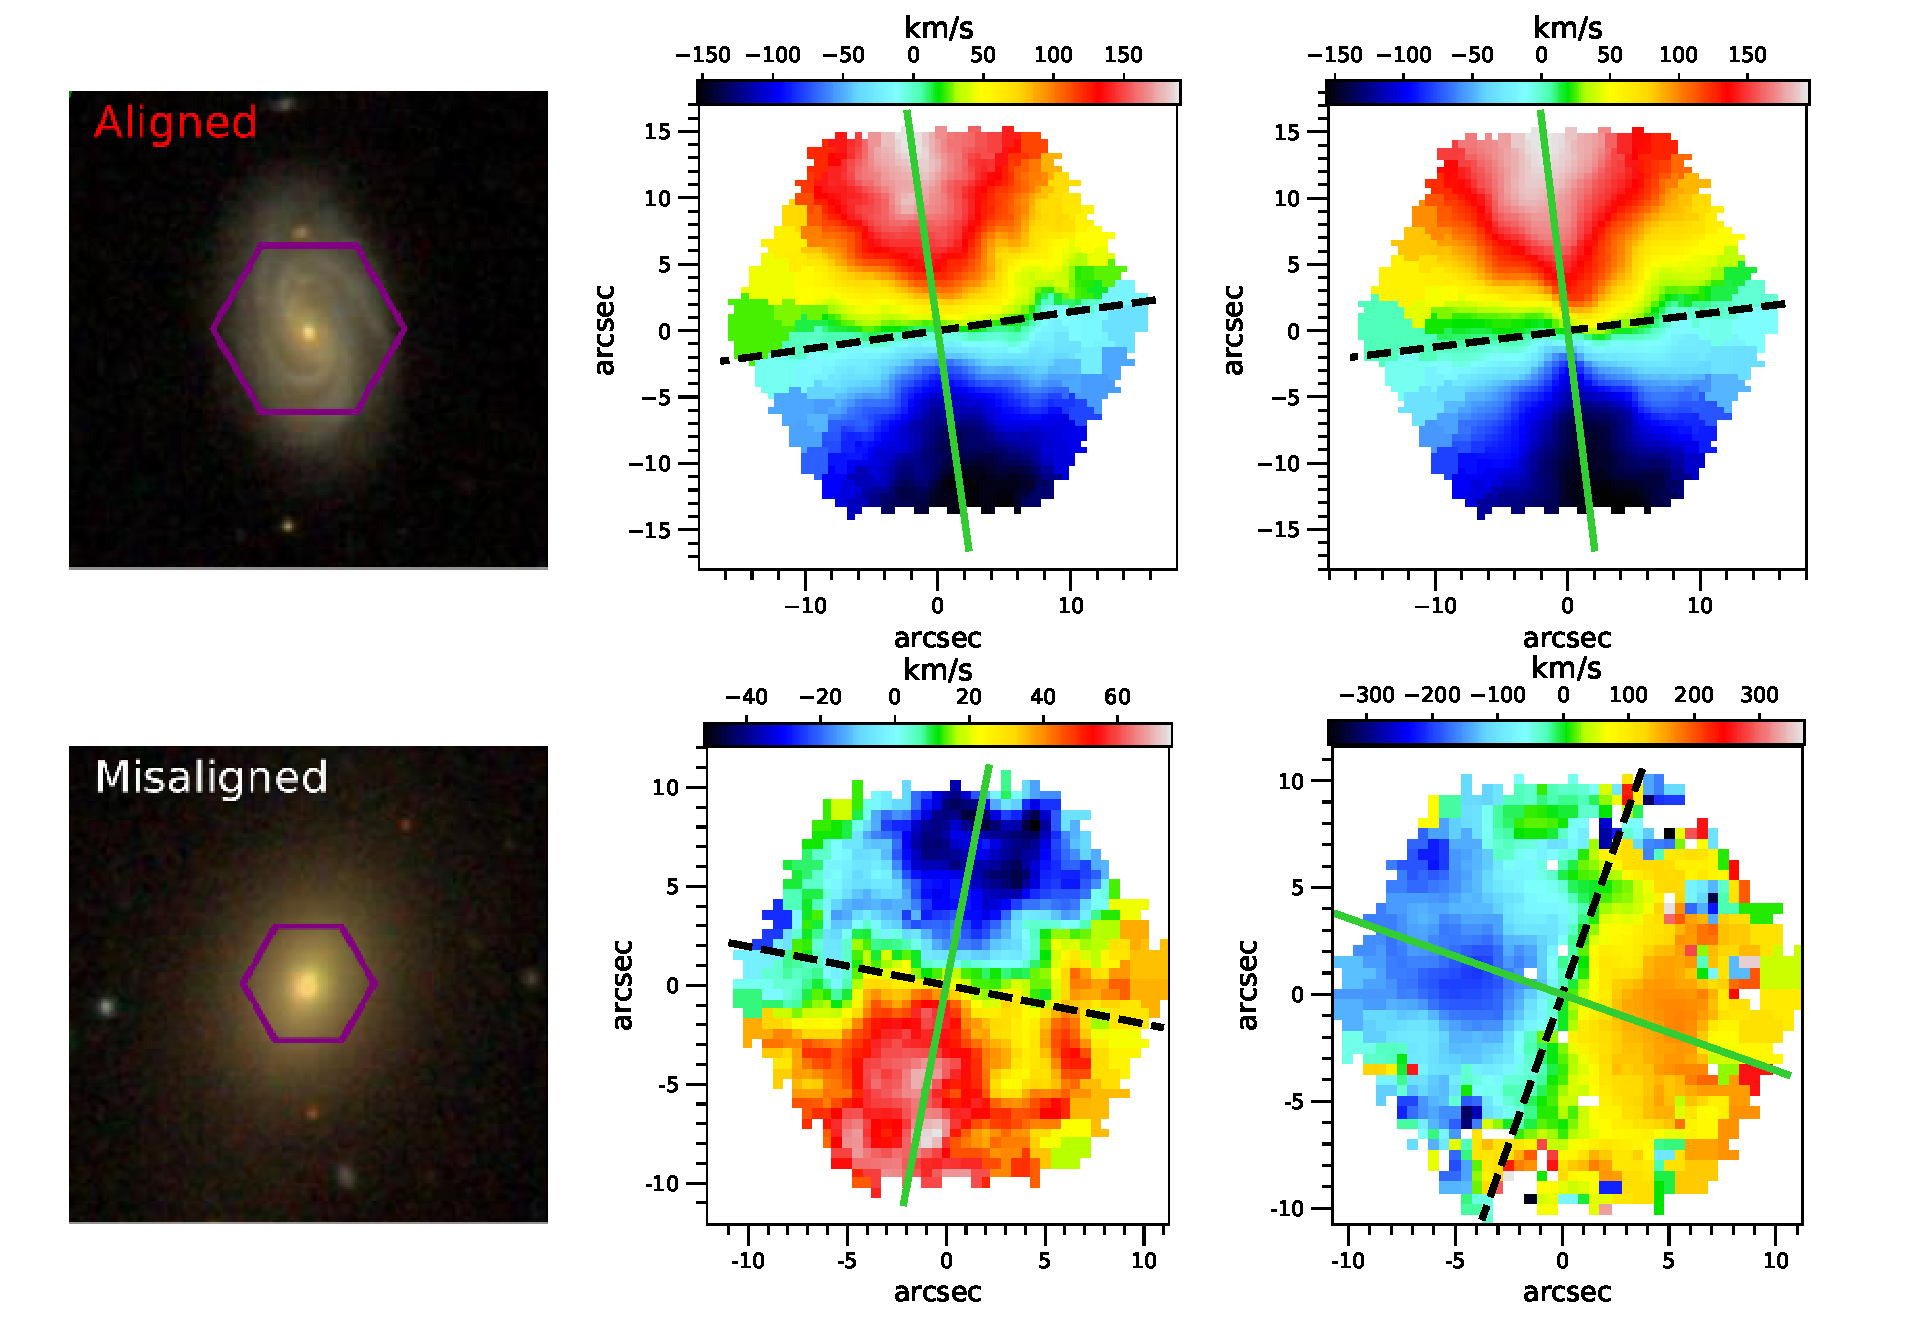
\includegraphics[width=0.8\linewidth]{thesis/latex/misalignment_MaNGA/cutout_wIFU_revised.pdf}
    \caption[Examples of a kinematically aligned (top) and misaligned (bottom) galaxy defined by $\Delta$PA.]{Examples of a kinematically aligned (top) and misaligned (bottom) galaxy defined by $\Delta$PA. From left to right, the panels show (i) the original SDSS cutout of surrounding field with the MaNGA IFU footprint overlaid in purple, (ii) stellar velocity field and (iii) $H\alpha$ (gas) velocity field. The velocity fields are marked by a defined PA (green solid line) and axis of rotation (black dashed line). The galaxy in the bottom row is misaligned due to it having $\Delta$PA > 30$^{\circ}$. The colour-bars represent the velocity fields in km/s and the galaxies are orientated so that up corresponds to North and right to East.}
    \label{fig:cutout_wIFU}
\end{figure*}

To improve the reliability of the PA fit, we apply a few additional filters to the velocity fields. While foreground stars are flagged within observations, background/small neighbouring galaxies can remain within the IFU footprint. This is a problem for fitting a global position angle since it naturally interprets other material as part of the target galaxy's observation and interpolates between the regions. We remove all disconnected regions smaller than $10\%$ of the target galaxy's footprint. In addition we sigma clip the velocity field and remove all spectral pixels (spaxels) above a $3\sigma$ threshold.

Our choice to take $\Delta$PA > 30$^{\circ}$ as significantly kinematically misaligned is a conservative selection to ensure we are selecting galaxies undergoing external interaction. There is evidence to suggest that accretion drives misalignment past $\Delta$PA = 30$^{\circ}$. \citet{lagos2015} found that using solely galaxy mergers as the source for misaligned cold gas only predicts 2\% of ETGs to have $\Delta$PA > 30$^{\circ}$ using GALFORM, in comparison with the misaligned field ETG fraction found in ATLAS\textsuperscript{3D} of 42 $\pm$ 6\%  \citep{davis2011a}. This puts a lower level of importance on gas accretion. Our choice can be justified as follows. Firstly, we are using ionized gas as a proxy for the distribution and accretion of cold gas. \citet{davis2011a} find that the typical difference between the PAs of cold gas (CO) and ionized gas can be described by a Gaussian distribution centred on 0 with a standard deviation of 15$^{\circ}$ for 38 CO bright galaxies in ATLAS\textsuperscript{3D}. While indicating ionized gas is a reasonable estimator for cold gas, splitting $\Delta$PA = 30$^{\circ}$ accounts for the scatter in this relationship. Secondly, this should avoid spurious misalignments arising from errors in the fit of $\Delta$PA. While our model errors are low, they are likely an underestimation since they do not include more complex motions. However, selecting a lower split in $\Delta$PA would only be affected by the increased likelihood of internal processes being dominant, rather than the inaccuracy of fitting. Any threshold in $\Delta$PA becomes a trade off between sample size and contamination probability. Altering our cut in $\Delta$PA to be 20$^{\circ}$, 40$^{\circ}$ or similar does not change any of the conclusions drawn in this chapter.

\subsection{Error estimation}
It is an important point to constrain the errors of our PA fits, so we can reliably trust cuts in $\Delta$PA to select galaxies which are significantly kinematically misaligned and hence have had external interaction. Here, we construct two component model velocity maps for each stellar and gas component of every MPL-6 observation in order to estimate typical errors on $\Delta$PA from \texttt{FIT\_KINEMATIC\_PA} for the MaNGA sample. \red{MPL-6 corresponds to a total of 4633 unique galaxy observations.}

Errors using the \texttt{FIT\_KINEMATIC\_PA} routine have been previously estimated for molecular gas velocity fields in ATLAS\textsuperscript{3D} \citep{davis2011a}. Model velocity fields with a known PA were constructed using an empirical galaxy rotation curve and combined with Gaussian noise matched to the signal-to-noise ratio of the data. A typical scatter of $\approx10^{\circ}$ was found due to varying inclination and angular resolution for the velocity fields.

\subsubsection{Circular velocity}
To find the typical error on $\Delta$PA for galaxies in MaNGA, we create model velocity maps for both the stellar and gas components of each MPL-6 observation. In each instance the basic construction of the model follows Section 4 of \citet{krajnovic2006}. Each velocity field comprises of a two-component Hernquist potential which provides a basic circular velocity given by,
\begin{equation}
\mathrm{V_c = \frac{\sqrt{GMr}}{r+r_0}}
\end{equation}
where $G$ is the gravitational constant, $M$ is the total mass and $r_0$ is the core radius of each component respectively \citep{hernquist1990}. We use a two-component model to include the relative strengths of both disc and bulge each with distinct effective radii, $R_e$. We fix $r_0$ to be 5 and 15 (units: $arcsec$) and $\sqrt{GM}$ to be 850 and 1500 (units: $km s^{-1} arcsec^{1/2}) $ for the bulge and disc components respectively. These individual components are light weighted by model sersic flux profiles according to,
\begin{equation}
\mathrm{I(r) = I_0 e^{-\left(\frac{R}{R_e}\right)^{n_s}}}
\end{equation}
where $I_{0}$ is the peak flux and $n_s$ is the sersic index which is set to 1 and 4 for the disc and spheroidal components respectively. Since we do not have bulge-disc decompositions, we lack individual effective radii for both the bulge and disc components. Instead, we set the bulge and disc effective radii to be 0.5$R_e$ and 1.5$R_e$, where $R_e$ is the effective radius estimated by an elliptical petrosian fit taken from the NSA targeting catalogue. 

\subsubsection{Calibration}
For each MaNGA galaxy a basic velocity field model is constructed using this template. The axes of the model velocity field are then scaled according to the inclination, $i$, which is estimated from the $b/a$ ratio taken from the NSA catalogue and is also used to scale the fraction of rotational velocity along the line-of-sight. The velocity field for each component, ($j=bulge,disc$), in polar coordinates $(r,\phi)$ is then described by,
\begin{equation}
\mathrm{V(r,\phi) = \frac{I_{j}(r)}{I_{tot}(r)}V_{c}(r)\cos(\phi+\theta_{j})\sin(i)}
\end{equation}
where $\theta_j$ is the input kinematic position angle. We set $\theta_{bulge} = \theta_{disc}$ for simplicity, however, we do note that galaxies with more complex orbital motions may increase the typical error. The position angle for both bulge and disc is simply taken to be the opening angle of the galaxy (direction of major axis taken from NSA catalogue). 

In order to imitate a MaNGA observation, the model velocity field is sampled at the spatial resolution of the corresponding IFU bundle and projected into the original shape of the actual observation for H$\alpha$ and stellar maps respectively. Gaussian noise is drawn for each spaxel from a normal distribution with the standard deviation taken from the errors on the actual observation. In addition, these model velocity fields are then Voronoi binned to match the original observation.

Example stellar and H$\alpha$ velocity fields generated from these models are shown in Figure \ref{fig:sim_ifu} with comparison to the actual observation. As expected, the model velocity fields frequently recreate observations well but struggle to encompass more complex motion. For this reason, our models should make a reasonable prediction on the typical $\Delta$PA errors intrinsic to MaNGA observations.

\begin{figure}
    \centering
	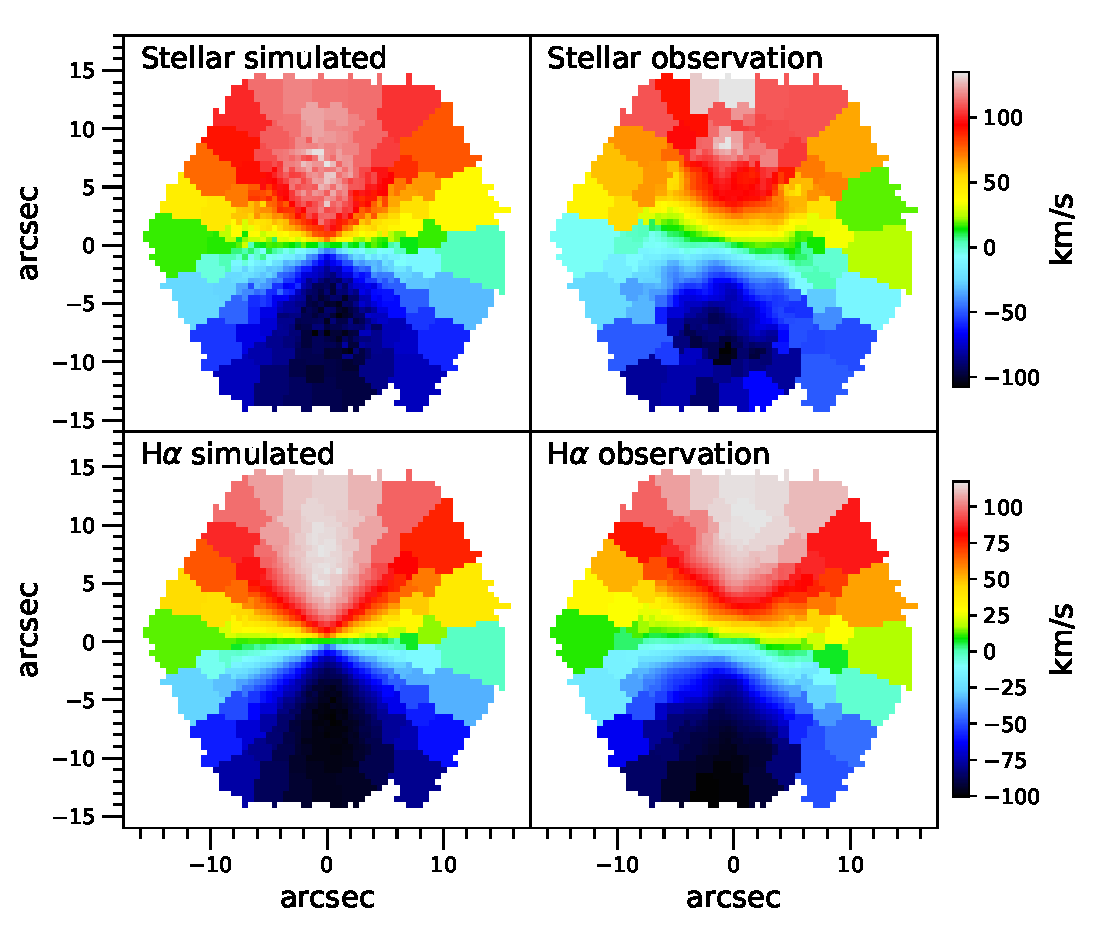
\includegraphics[width=0.7\linewidth]{thesis/latex/misalignment_MaNGA/obs_sim_IFU.pdf}
    \caption[Comparison velocity maps for simulation (left column) and observation (right column).]{Comparison velocity maps for simulation (left column) and observation (right column). Stellar (H$\alpha$) component velocity maps are shown on the top (bottom) row with the associated velocity colourbars.}
    \label{fig:sim_ifu}
\end{figure}

\subsubsection{Typical errors}
We construct model velocity fields for all non-critically flagged MPL-6 galaxies, inclusive of the $\Delta$PA sample used in this work. Figure \ref{fig:model_errors} shows the cumulative probability distribution for the range of $0-5^{\circ}$ where the majority of errors fall. We find that \texttt{FIT\_KINEMATIC\_PA} gives a typical combined (stellar and gas) mean error of $1.3^{\circ}$. While this is an underestimation of true $\Delta$PA errors for a sample of galaxies including those with more complex velocity fields, it is indicative that selecting a cut at $\Delta$PA = 30$^{\circ}$ should be robust to identifying galaxies with external interaction. \todo{Has python version of fit kinematic pa been updated to include this?}

\begin{figure}
    \centering
	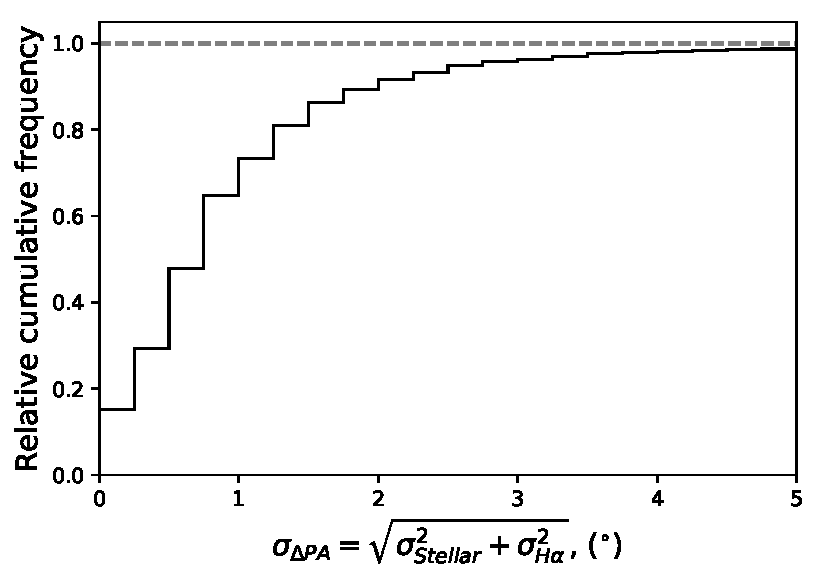
\includegraphics[width=0.6\linewidth]{thesis/latex/misalignment_MaNGA/cumulative_model_errors.pdf}
    \caption{Cumulative histogram of errors for fitting kinematic PA to model maps for the all non-critically flagged MPL-6 galaxy observations.}
    \label{fig:model_errors}
\end{figure}

\subsection{Visual Classification}
Global position angles are only well defined for coherently rotating velocity fields. Those with a decoupling between inner and outer regions due to warps or kinematically decoupled cores (KDCs) are poorly described by global PAs. To select a clean sample of galaxies with well defined global PAs, we visually classify all of the velocity fields after pre-processing and PA fitting. Both stellar and H$\alpha$ velocity fields are characterised into 3 categories;
\begin{itemize}
    \item Dominant coherent rotation and well defined PA.
    \item Dominant coherent rotation but with more noise or more complex motion resulting in a usable PA fit but with higher typical errors. Highly inclined velocity fields with a higher likelihood of inaccurate PAs fits are included in this category. 
    \item Do not use.
\end{itemize}

Kinematic features are also identified. Both stellar and H$\alpha$ velocity fields are classified into;
\begin{itemize}
    \item Kinematically decoupled core (i.e. those with a central component that rotates in a different direction ($> 30^{\circ}$) with respect to the overall galaxy rotation).
    \item Warp (velocity field of central region is warped with respect to outskirts. This may be due to a bar, oval shaped structures in the disc (oval distortions) or accretion of fresh material with different angular momentum to the bulk rotation).
    \item Merger (ongoing merger or neighbour identified within IFU. Only those with obvious disruption are followed up in photometry).
    \item No features.
\end{itemize}
The majority of those with kinematic features have poorly defined global PAs and hence are flagged as do not use for the previous flag. The galaxies we refer to as `warped' represents a combination of galaxies with bars, oval distortions and differential rotation in the disc \citep[e.g.][]{barrera2014}. We direct the reader to \citet{stark2018} for an approach to separate the galaxies we refer to as warps. In this work, we enforce axisymmetry for our sample and hence make no use of galaxies that have significant variations in their PA as a function of radius.

For studies of quenching it may be useful to consider galaxies that have defined stellar rotation but lack coherent motion in the ionized gas. For galaxies that have usable PAs for the stellar velocity but unusable PAs for the ionized gas, we define a further classification of the gas velocity field;
\begin{itemize}
    \item Depletion (seen as empty spaxels signifying lack of gas, usually in central regions)
    \item No clear rotation (map has no clear rotation or is noise dominated)
    \item Partial rotation (partial coherent rotation in the velocity field, however there are significant regions with incoherent motion or noise domination)
    \item No clear characteristics/ No gas.
\end{itemize}
We note there is a clear overlap between the classifications for depletion and no clear rotation, since velocity fields are often a combination of these two features. 
%The total numbers for each classification in each category are summarised in Table \ref{tab:kin_class}. 
Examples of PA fits (see \S\ref{sec:def_kin_mis} for calculation) with the associated photometry for various kinematic classifications is given in Figure \ref{fig:mis_grid}. Examples of galaxies that are kinematically aligned, misaligned, have a stellar kinematically decoupled core, have a warped H$\alpha$ velocity field and have clear stellar rotation but depleted ionized gas/ no rotation are shown respectively.

\begin{figure*}
    \centering
	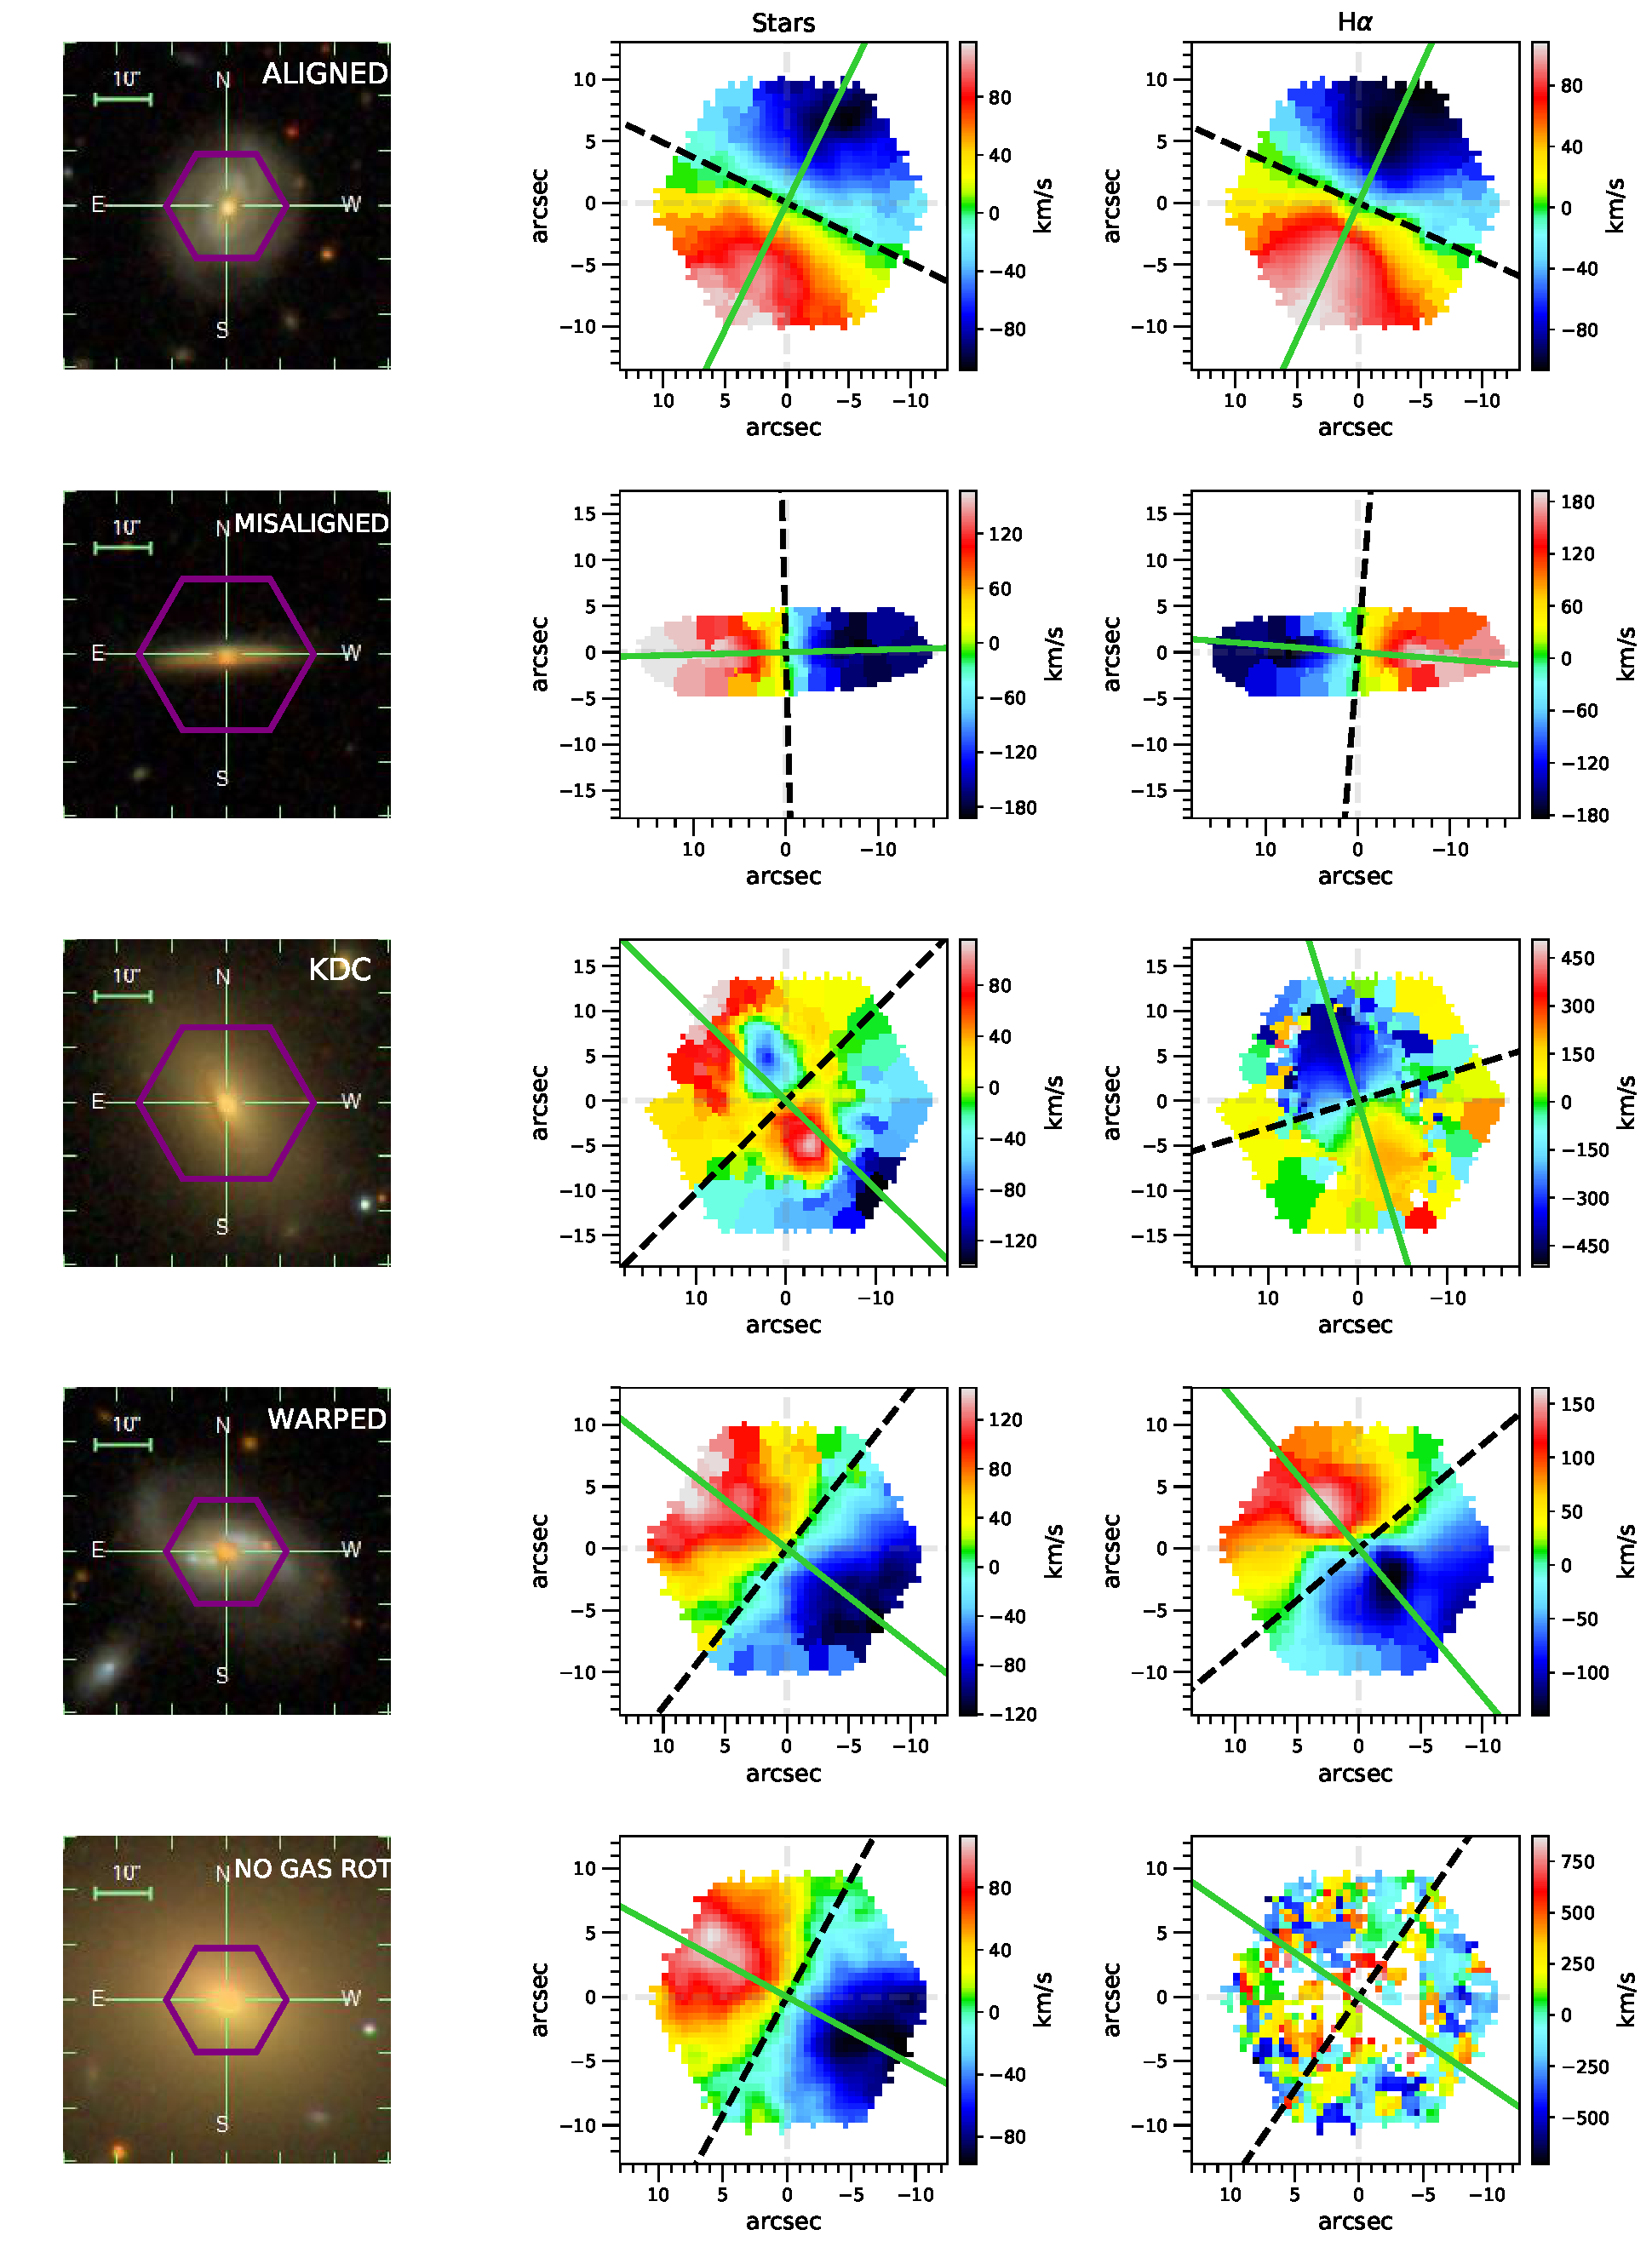
\includegraphics[width=0.93\linewidth]{thesis/latex/misalignment_MaNGA/misalignment_grid.pdf}
    \caption{Examples of PA fits for galaxies with different kinematic classifications. For each galaxy (row), we show the photometry taken from SDSS with the MaNGA IFU observation footprint overlaid in purple (left), the stellar velocity field (middle) and the H$\alpha$ velocity field (right). The kinematic PA fits (see \S\ref{sec:def_kin_mis}) are shown on the velocity fields (green solid line) with the axis of rotation (black dotted line). The kinematic classifications from top to bottom are; (a) PLATEIFU: 7958-6101, kinematically aligned near face on; (b) PLATEIFU: 8465-12704, counter-rotating near edge on; (c) PLATEIFU: 9868-12704, with a KDC in the stellar velocity; (d) PLATEIFU: 8252-6103, with a warped H$\alpha$ velocity field with respect to the stellar; (e) PLATEIFU: 10219-6102, with a centrally depleted/missing H$\alpha$ velocity field but coherent rotation in the stellar.}
    \label{fig:mis_grid}
\end{figure*}

\section{Data} \label{sec:data_obs}
This section describes the catalogues crossed matched with the MaNGA sample to seperate galaxies based on optical morphology and group membership.

\subsection{Morphology} \label{sec:morph_def_obs}
We classify the morphology of MaNGA galaxies through the formalism laid out by the citizen science project; GalaxyZoo2 \citep[GZ2;][]{willett2013}. GZ2 provides visually identified morphologies (and also measures finer morphological features e.g. bars, bulge size and edge-on discs) for 304,122 galaxies drawn from SDSS. GZ2, however, is not complete for the MaNGA sample and has been combined with an unpublished version; GalaxyZoo4 to provide a consistent set of definitions for all MaNGA targets (see \url{https://www.sdss.org/dr15/data_access/value-added-catalogs/?vac_id=manga-morphologies-from-galaxy-zoo}). 

In a nutshell, GZ2 provides morphological classification through a decision tree of questions. Further questions are dependent on the answer to the previous to characterise a certain morphological type and identify finer features (see Figure 1 in \citet{willett2013} for this flowchart). From this, a table of vote fractions for each question combined with the total number of votes dictate a reliably sampled galaxy population with a set of desired morphological features. Votes by individuals are debiased (weighted) based on their reliability in comparison to known answers to the questions.

The first question in the decision tree 'Is the galaxy smooth and rounded with no sign of a disc?', allows categorisation into broad ETGs and LTGs. We select galaxies with a debiased vote fraction > 0.7 for smooth to be ETGs and galaxies with a debiased vote fraction of > 0.7 for disc or features to be LTGs. Defining an exact population of lenticular galaxies (S0s) is tricky through public classifications. LTGs, however, can be separated based on the dominance of the bulge with respect to the disc in GZ2 through the question 'How prominent is the central bulge, compared with the rest of the galaxy?'. \citet{willett2013} demonstrate a strong correlation between bulge dominance as defined per this question and expert classifications of T-type \citep{nair2010}. Equation 19 of \citet{willett2013} provides a linear mapping from GZ2 bulge classification to expert defined morphological T-type. Care must be taken in using this linear mapping \citep[see discussion in][]{willett2013}, however, this should be a reasonable parameterisation to coarsly separate LTGs into earlier-type (S0 - Sa) and later-type spirals (Sb - Sd). We split our LTG population at T-type = 3, to give two morphological categories; S0-Sas and Sb-Sds in addition to pure ETGs.
% We split our LTG population at T-type = 3, to give three morphological categories along with pure ETGs. 

The estimates of gas mass used here for MaNGA are derived from the Pipe3D pipeline \citep{pipe3Da, pipe3Dvac}, which uses dust attenuation within the footprint of the IFU, which methodology is described in \citet{barrera2018}.

\subsection{Group membership} \label{sec:group_def}
\red{either put full description here or in halo assembly section.}
To investigate different pathways leading to kinematic misalignment, we must separate galaxies into centrals and satellites. We identify groups with an adaptive halo-based group finder of \citet{yang2005,yang2007} and with improved halo mass assigning techniques \citep[see;][for details and application to SDSS]{lim2017}. In a nutshell, the group finder uses either the stellar mass or luminosity of central galaxies in addition with the $\mathrm{n^{th}}$ brightest/most massive satellite as proxies for halo mass. Galaxies are assigned to groups through an iterative process, where halo properties such as halo size and velocity dispersion are updated until membership converges. 

% For groups that are outside of the redshift limit where groups are complete final halo masses are assigned through abundance matching. Those incomplete are assigned halo masses based on the ranking between halo mass and the proxy found at the final iteration of the group finder.
% The performance of the group finder has been tested on realistic mock catalogues, showing that the halo masses of individual haloes are consistent with the true mass with a typical scatter of $\sim$0.2 dex. This scatter is similar to the commonly used group finder of \citet{yang2007}, however extends uniformly to halo masses 0.7 dex lower. 

% For this work, we use the stellar mass based halo mass proxy for the SDSS main sample. 
\citet{lim2017} do not apply the group finder to the thin strips in the Southern Galatic Cap of SDSS main due to incomplete groups resulting from close proximity to borders. MaNGA galaxies in these strips are therefore unclassified by the group finder, resulting in 5088 matched galaxies with group membership classifications into central or satellite. 

\section{Results} \label{sec:results_obs}
\red{redefine NGRs}
We divide our MaNGA $\Delta$PA defined population at $\Delta$PA = 30$^{\circ}$ into aligned and misaligned. In the following, we also consider galaxies with defined stellar PAs but undefined H$\alpha$ due to central depletion or incoherent rotation/dispersion domination (no gas rotation; NGRs). Figure \ref{fig:delPA_stelM} shows the distribution of stellar mass for these three populations. We see no significant difference between the aligned and misaligned galaxies, however NGRs appear to be slightly more massive. \citet{graham2018} previously demonstrated the tight correlation between stellar angular momentum and stellar mass for MaNGA ($\sim$2300 galaxies). Since NGRs and misaligned galaxies are slightly higher mass, it could be expected that they are typically less rotationally supported with respect to the $\Delta$PA defined populations. 

\begin{figure}
    \centering
	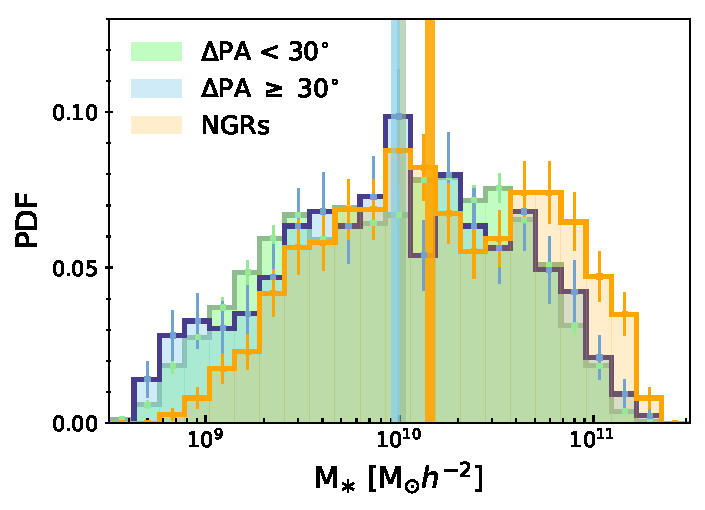
\includegraphics[width=0.7\linewidth]{thesis/latex/misalignment_MaNGA/delPA_stelM.pdf}
    \caption{Probability density distributions of stellar mass, $\mathrm{(M_{\ast}/M_{\odot})}$ for aligned galaxies ($\Delta$PA < 30$^{\circ}$) shown in green, those with high misalignment ($\Delta$PA > 30$^{\circ}$) are in blue and NGRs are in orange. Each histogram is given with Poisson errors on each bin. The vertical lines denote the corresponding distribution's median. NGRs are typically at higher stellar mass than those with aligned star and gas rotation.}
    \label{fig:delPA_stelM}
\end{figure}

Here we use the luminosity weighted stellar angular momentum estimator, $\mathrm{\lambda_R}$, taken directly from Equation 1 in \citet{emsellem2007} as
\begin{equation}
\mathrm{\lambda_{R} \equiv \frac{\langle R | V | \rangle}{ \langle R \sqrt{ V^{2} + \sigma^{2} } \rangle } = \frac{ \Sigma_{ n = 1 }^{ N } F_{ n } R_ { n } \left| V_{ n } \right| }{ \sum_{ n = 1 }^{ N } F_{n} R_{ n } \sqrt{ V_{ n }^{ 2 } + \sigma_{ n }^{ 2 } } }.}
\end{equation}
$\mathrm{\lambda_R}$ is calculated from summing over N pixels in the IFU observation within the radius of interest, $\mathrm{R}$. $\mathrm{F_{n}}$, $\mathrm{V_{n}}$ and $\mathrm{\sigma_{n}}$ are the flux, line of sight velocity and line of sight velocity dispersion of the $\mathrm{n^{th}}$ pixel. Here we present all measures of $\mathrm{\lambda_R}$ encompassing a radius of $\mathrm{1.5R_e}$ weighted by $r-$band flux. We also take the ellipticity to be $\mathrm{\epsilon = 1 - b/a}$ where $a$ and $b$ are the major and minor axes of the galaxy estimated from the NASA Sloan Atlas catalogue \cite[used for target selection in MaNGA;][]{blanton2011}.

Figure \ref{fig:delPA_lambda_Re}, shows $\mathrm{\lambda_R}$ vs $\mathrm{\epsilon}$ for all $\Delta$PA defined galaxies and the medians for the aligned, misaligned and NGR samples. The black solid line overlaid shows the slow rotator regime (enclosed in bottom left). The fast/slow rotator classification refers to whether a given galaxy's rotation can be considered regular (circular velocity) or exhibits dispersion dominated motion \citep[][]{emsellem2007}. Kinematically aligned galaxies reside at preferentially higher $\mathrm{\lambda_R}$ and ellipticity with respect to NGRs. This is indicative of the dispersion dominance over rotation for disrupted gas poor and typically higher mass galaxies that we see in our NGR sample. Interestingly, kinematically misaligned galaxies also typically reside close to the slow rotator regime. In addition, the same qualitative trends are seen (i.e. misaligned and NGR galaxies have lowered angular momentum with respect to the aligned) are seen if this plot is made for ETGs, S0-Sas or Sb-Sds alone. 

\begin{figure}
    \centering
	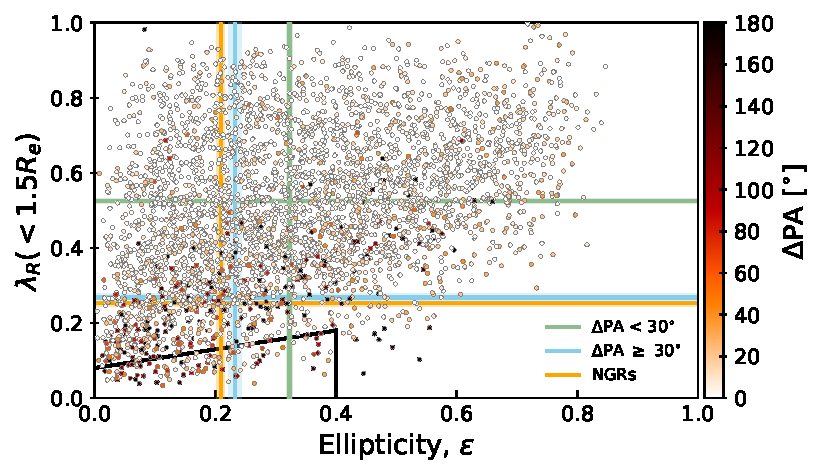
\includegraphics[width=\linewidth]{thesis/latex/misalignment_MaNGA/delPA_lambda_Re.pdf}
    \caption{$\lambda_R$ within 1.5$\mathrm{R_e}$ against ellipticity, $\epsilon$ for all galaxies with defined $\Delta$PA. The individual points are for all $\Delta$PA defined MaNGA galaxies coloured by $\Delta$PA according to the colorbar. Medians for kinematically aligned ($\Delta$PA < 30$^{\circ}$), misaligned ($\Delta$PA > 30$^{\circ}$) and NGRs are shown by the green, light blue and orange lines respectively. The lighter shade around each line corresponds to the standard error. Aligned galaxies reside more typically in the fast rotator regime with higher $\lambda_R$ and $\epsilon$, whereas misaligned galaxies and NGRs reside closer to the slow rotator regime. The same qualitative trends are found if this plot is made for ETGs, S0-Sas or Sb-Sds alone.}
    \label{fig:delPA_lambda_Re}
\end{figure}

In Figure \ref{fig:delPA_gasM} we show the distribution of gas masses for the aligned, misaligned and NGRs. We see a clear trend of lower gas mass going from kinematically aligned galaxies to misaligned galaxies to NGRs. We note that the majority ($\sim$80\%) of NGRs do not contain enough gas to have a measured gas mass from the routine of Pipe3D, so the distribution shown is a hard upper limit on the gas that these galaxies contain. We note that these trends remain qualitatively the same when considering the distributions for ETGs, S0-Sas and Sb-Sds individually.

\begin{figure}
    \centering
	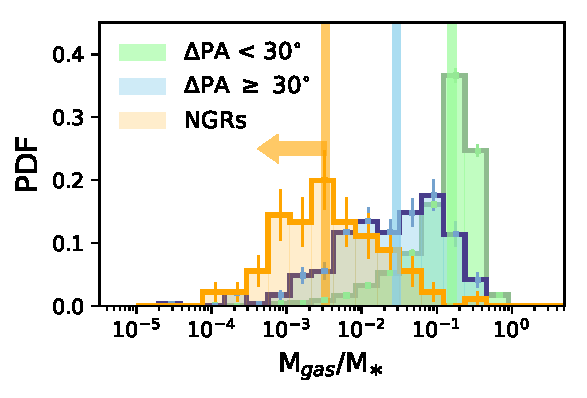
\includegraphics[width=0.8\linewidth]{misalignment_MaNGA/gas_mass_normed_all.pdf}
    \caption{Probability density distributions of gas mass fraction, $\mathrm{(M_{gas}/M_{\ast})}$ for aligned galaxies ($\Delta$PA < 30$^{\circ}$) shown in green, those with high misalignment ($\Delta$PA > 30$^{\circ}$) in light blue and NGRs in orange. Each histogram is given with Poisson errors on each bin. The vertical lines denote the corresponding distribution's median. The majority of NGRs do not have detectable gas masses and therefore the distribution shown should be considered as upper bound.}
    \label{fig:delPA_gasM}
\end{figure}

The similarity in stellar angular momentum between the NGRs and kinematically misaligned galaxies could indicate that they are from the same evolutionary sequence. A key component in decoupling star-gas rotation in simulations is a significant gas loss followed later by the accretion of material with misaligned angular momentum \citep[][]{vdvoort2015, starkenburg+19}. This gas loss can happen due to interactions from neighbouring galaxies which strips gas or through ejection due to black hole feedback.

In \red{section halo assembly} \citet{duckworth2019a}, it was shown that kinematic decoupling shows little relationship with distance to filamentary structure. This could point to stripped/ejected material being re-accreted as a potential source of misalignment between star and gas rotation. Some NGRs could therefore represent an earlier timestamp before this material is re-accreted. Not all NGRs would necessarily re-accrete gas, meaning that some would remain quenched (and hence would not become misaligned in the future) potentially explaining the differences we see in stellar mass distributions of NGRs and misaligned. In this scenario, it would suggest that re-accretion of new material does not significantly alter the stellar angular momentum content going from NGRs to misaligned.

\subsection{Morphology}
We now sub-divide the total population by morphology into ETGs, S0-Sas and Sb-Sds as defined in \S\ref{sec:morph_def}. Figure \ref{fig:morph_PA}, shows the distributions for each category. We find that for all morphological types, galaxies are most commonly aligned with strong peaks below $\Delta$PA $\sim 30^{\circ}$. ETGs show a flatter distribution than their later counterparts, as the most likely to exhibit misalignment. LTGs show deeper drop-offs above $\Delta$PA $\sim 40^{\circ}$, with a boost around $\Delta$PA = 180$^{\circ}$, seen most strongly for the Sb-Sds. We quantify the overall misalignment fractions in the first column of Table \ref{tab:mega_table}. Our errors are estimated by binomial counting errors so that $\mathrm{\sigma = \sqrt{p(1-p) / M}}$ where $\mathrm{p = N/M}$ with $\mathrm{N}$ being the number of misaligned galaxies and $\mathrm{M}$ the total number of galaxies for the category.

This morphological difference in misalignment is likely a result of several factors. Gas rich LTGs have typically higher specific angular momentum, and hence, require a higher magnitude gas inflow/outflow with different angular momentum to disrupt rotation and create misalignment. Conversely, ETGs are more dispersion dominated and gas poor enabling smaller gas in-flows (or outflows) to create a kinematic misalignment. 

These results are reasonably consistent with previous findings of 36$\pm$5\% (of 260 galaxies) of ETGs that are misaligned in ATLAS\textsuperscript{3D} and in SAMI (45$\pm$6\% of 36 pure ellipticals, 5$\pm$1\% in 221 pure late spirals) \citep[][]{davis2011, bryant2019}. We note that our ETG misalignment fraction ($\sim$28\%) is lower than these previous findings and holds a slight tension with \citet{bryant2019}. Possible reasons for the differences may be due to morphology definition, stellar mass distribution or simply sample size. We note that enforcing stricter thresholds for morphology classifications doesn't change our misaligned fractions pointing to a likely difference in mass distributions or our increased sample size. 

\begin{table*}
\begin{tabular}{lllll}
\hline
        &  & All & Centrals & Satellites \\
\hline
All galaxies & $\Delta$PA defined &  3798 &  2185 &  1007 \\
& $\Delta$PA $\geq 30^{\circ}$ &  420 (11.1$\pm$0.5\%) &  251 (11.5$\pm$0.7\%) &  102 (10.1$\pm$1.0\%) \\
& NGR & 742 &  334 &  324 \\

ETGs & $\Delta$PA defined & 301 & 204 & 97 \\
& $\Delta$PA $\geq 30^{\circ}$ & 84 (27.9$\pm$2.6\%) & 60 (29.4$\pm$3.2\%) & 24 (24.7$\pm$4.4\%)  \\
& NGR & 231 & 140 & 91 \\

S0 - Sas & $\Delta$PA defined & 677 & 483 & 194 \\
& $\Delta$PA $\geq 30^{\circ}$ &  66 (9.7$\pm$1.1\%) & 49 (10.1$\pm$1.4\%) & 17 (8.8$\pm$2.0\%) \\
& NGR & 100 & 44 & 56 \\

Sb - Sds & $\Delta$PA defined & 1634 & 1112 & 522 \\
& $\Delta$PA $\geq 30^{\circ}$ & 88 (5.4$\pm$0.6\%) & 58 (5.2$\pm$0.7\%) & 30 (5.7$\pm$1.0\%) \\
& NGR & 107 & 32 & 75 \\

\end{tabular}
\caption{Total number of galaxies used in this study for each of $\Delta$PA defined sample, of those that are kinematically misaligned and those that have well defined stellar rotation but incoherent gas (NGR). These are defined for both splitting on morphology (rows) and group membership (columns). For those that are kinematically misaligned ($\Delta$PA $\geq 30^{\circ}$), the percentage with respect to all those with $\Delta$PA measurements for the sub-category is shown. The uncertainties quoted are binomial counting errors.}
\label{tab:mega_table}
\end{table*}

The boost in the PDF around 180$^{\circ}$ of Figure \ref{fig:morph_PA} suggests that near counter-rotation is a stable state for galaxies. This is seen most prominently in Sb-Sds with a clear upwards trend in the PDF from $\sim$140$^{\circ}$. A possible explanation is that these rotation dominated galaxies host strong stellar torques, which act to realign gas at intermediate misalignments ($30^{\circ} < \Delta$PA $ < 150^{\circ}$) on much faster timescales than in ETGs. Counter-rotators, however, remain stable and hence contribute proportionally higher to the misaligned distribution, in comparison to those at intermediate misalignments which settle towards alignment or counter-rotation.

Interestingly galaxies that exhibit near-counter rotation ($\Delta$PA $\geq$ 150$^{\circ}$) have similar stellar angular momentum to the general misaligned population ($\Delta$PA $\geq$ 30$^{\circ}$), significantly lower than the aligned counterparts. This holds true for all morphologies. \citet{chen2016} previously highlighted the boost in star formation in central regions for counter-rotating LTGs. As suggested, this could be a natural result of cancellation of angular momentum leading to increased in-flows to central regions. Our finding of lowered angular momentum in the counter-rotators (with respect to the co-rotators) supports this claim.

\begin{figure}
	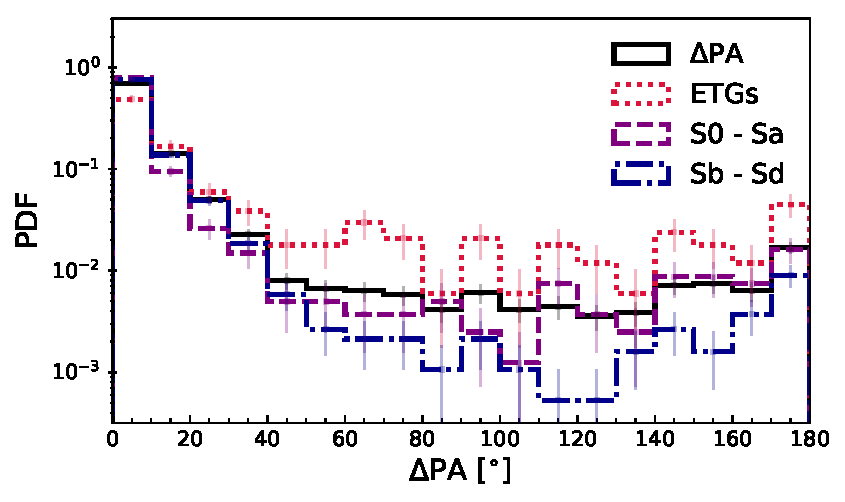
\includegraphics[width=\linewidth]{thesis/latex/misalignment_MaNGA/delPA_morph.pdf}
    \caption{Probability density distributions of kinematic misalignment as defined by $\Delta$PA split on morphology. The probability density distribution is normalised to 1 and shown in log scale. Distributions for the total population, ETGs, S0/Sa and Sb-Sds are shown by black solid, dotted red, dashed purple and dot-dashed blue lines respectively. Earlier type galaxies are more likely to be misaligned than later type galaxies.}
    \label{fig:morph_PA}
\end{figure}

Due to the relationship between stellar mass, morphology and specific angular momentum \citep[e.g.][]{cortese2016}, it might be expected that misaligned galaxies should be at higher stellar mass due to their lower $\mathrm{\lambda_{R}}$ with respect to the aligned \citep[see also;][]{bryant2019}. Surprisingly for the overall population we see little difference, however, splitting on morphology as shown in Figure \ref{fig:morph_stelM} reveals individual trends. Misaligned ETGs (and NGRs) are more massive than the aligned counterparts most likely indicative that misaligned galaxies have had richer merger histories. The opposite trends are seen for both S0-Sas and Sb-Sds with kinematically aligned galaxies being of typically higher mass than the misaligned. This could be indicative that the pathways leading to misalignment are different as a function of morphology.

\begin{figure}
    \centering
	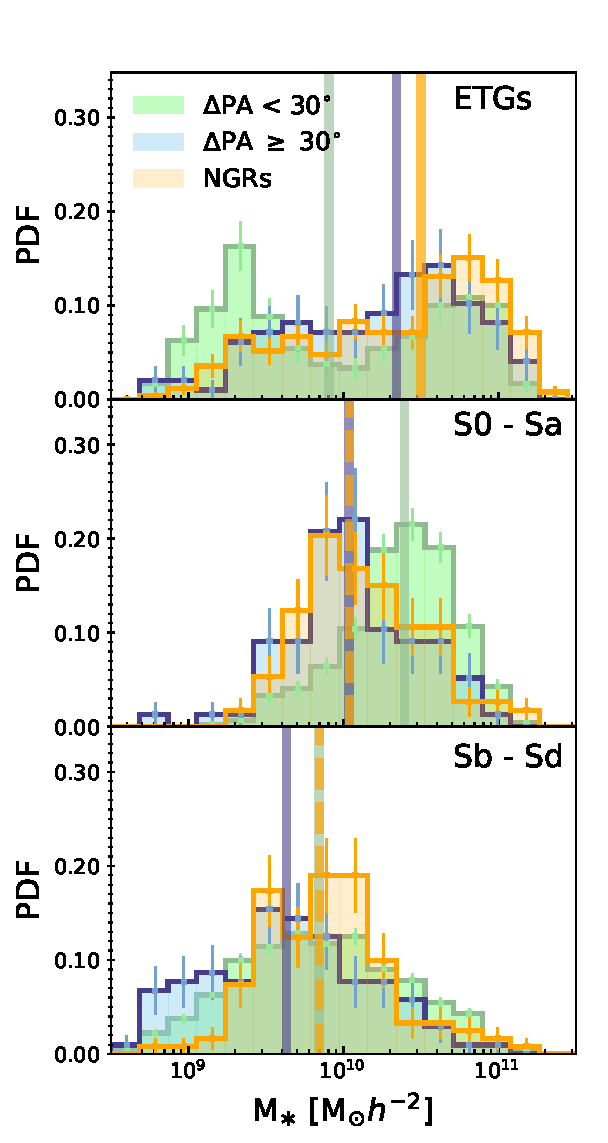
\includegraphics[width=0.5\linewidth]{thesis/latex/misalignment_MaNGA/delPA_stelM_morph_nsa.pdf}
    \caption{Probability density distributions of stellar mass, $\mathrm{(M_{\ast}/M_{\odot})}$ for aligned galaxies ($\Delta$PA < 30$^{\circ}$, misaligned galaxies ($\Delta$PA > 30$^{\circ}$) and NGRs for ETGs, S0-Sas and Sb-Sds (top to bottom). In each panel the aligned/misaligned are shown with solid lines with the aligned in the darker shade. NGRS are shown by dot-dashed lines. Each histogram is given with Poisson errors on each bin. The vertical lines denote the corresponding distribution's median. For ETGs, aligned galaxies are less massive than the misaligned sample. This trend, however, reverses for S0-Sas and Sb-Sds.}
    \label{fig:morph_stelM}
\end{figure}

\subsection{Group membership}
Group membership is important for dictating the evolution of a galaxy and hence we now sub-divide our population into centrals and satellites as described in \S\ref{sec:group_def}. Figure \ref{fig:group_morph_PA} (top panels) shows the $\Delta$PA distributions as in Figure \ref{fig:morph_PA}, but now split into centrals and satellites. Qualitatively the morphological trends remain however Table \ref{tab:mega_table} reveals that centrals (29.4$\pm$3.2\%) are slightly more likely to be misaligned than satellites (24.7$\pm$4.4\%) for ETGs. This is also potentially seen for the S0-Sbs (10.1$\pm$1.4\% for centrals vs 8.8$\pm$2.0\% for satellites), however we note that both fractions are within each other's errorbars.

\begin{figure*}
    \centering
	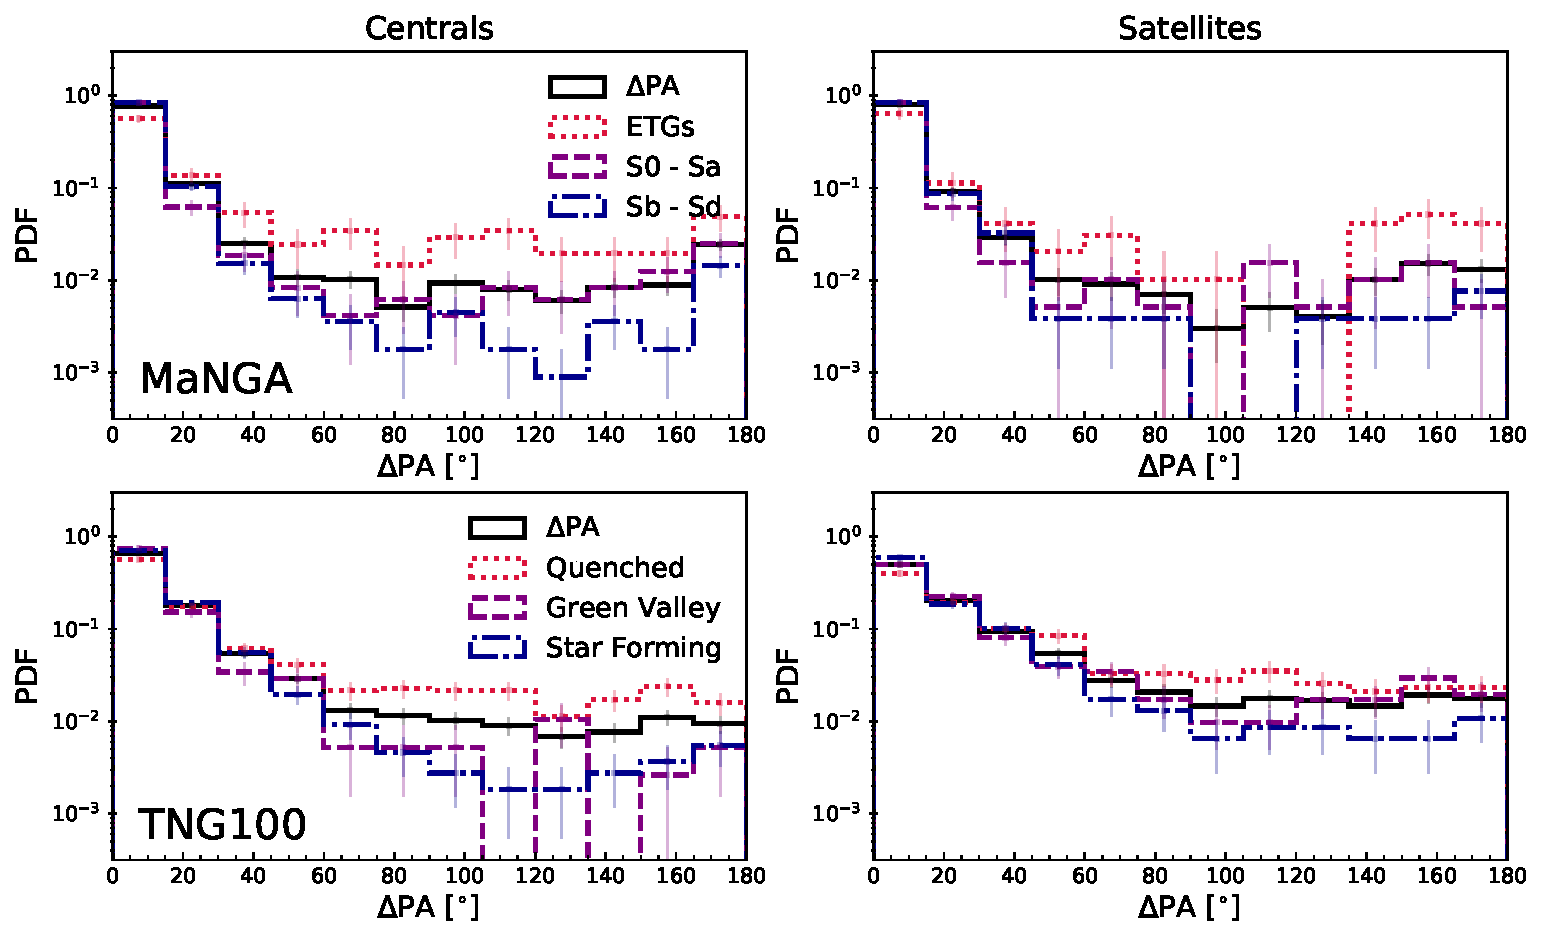
\includegraphics[width=\linewidth]{misalignment_MaNGA/MPL8_TNG_morph_group_PA.pdf}
    \caption{Same as Figure \ref{fig:morph_PA}, however split by group membership into centrals (left) and satellites (right). The top panel shows for the MaNGA sample and the bottom shows for the mock sample in TNG100. Morphology for TNG100 is categorised by the deviation of the galaxy's star formation away from the main sequence of galaxies in the whole of TNG100 (see \S\ref{sec:tng_results})}
    \label{fig:group_morph_PA}
\end{figure*}

Figure \ref{fig:group_morph_stelM} shows the stellar mass distribution for our samples but now additionally split into centrals and satellites. Again we find the same qualitative trends for both centrals and satellites; i.e. misaligned ETGs are more massive than their aligned counterparts whereas misaligned S0-Sas and Sb-Sds are less massive than those aligned.
\begin{figure*}
    \centering
	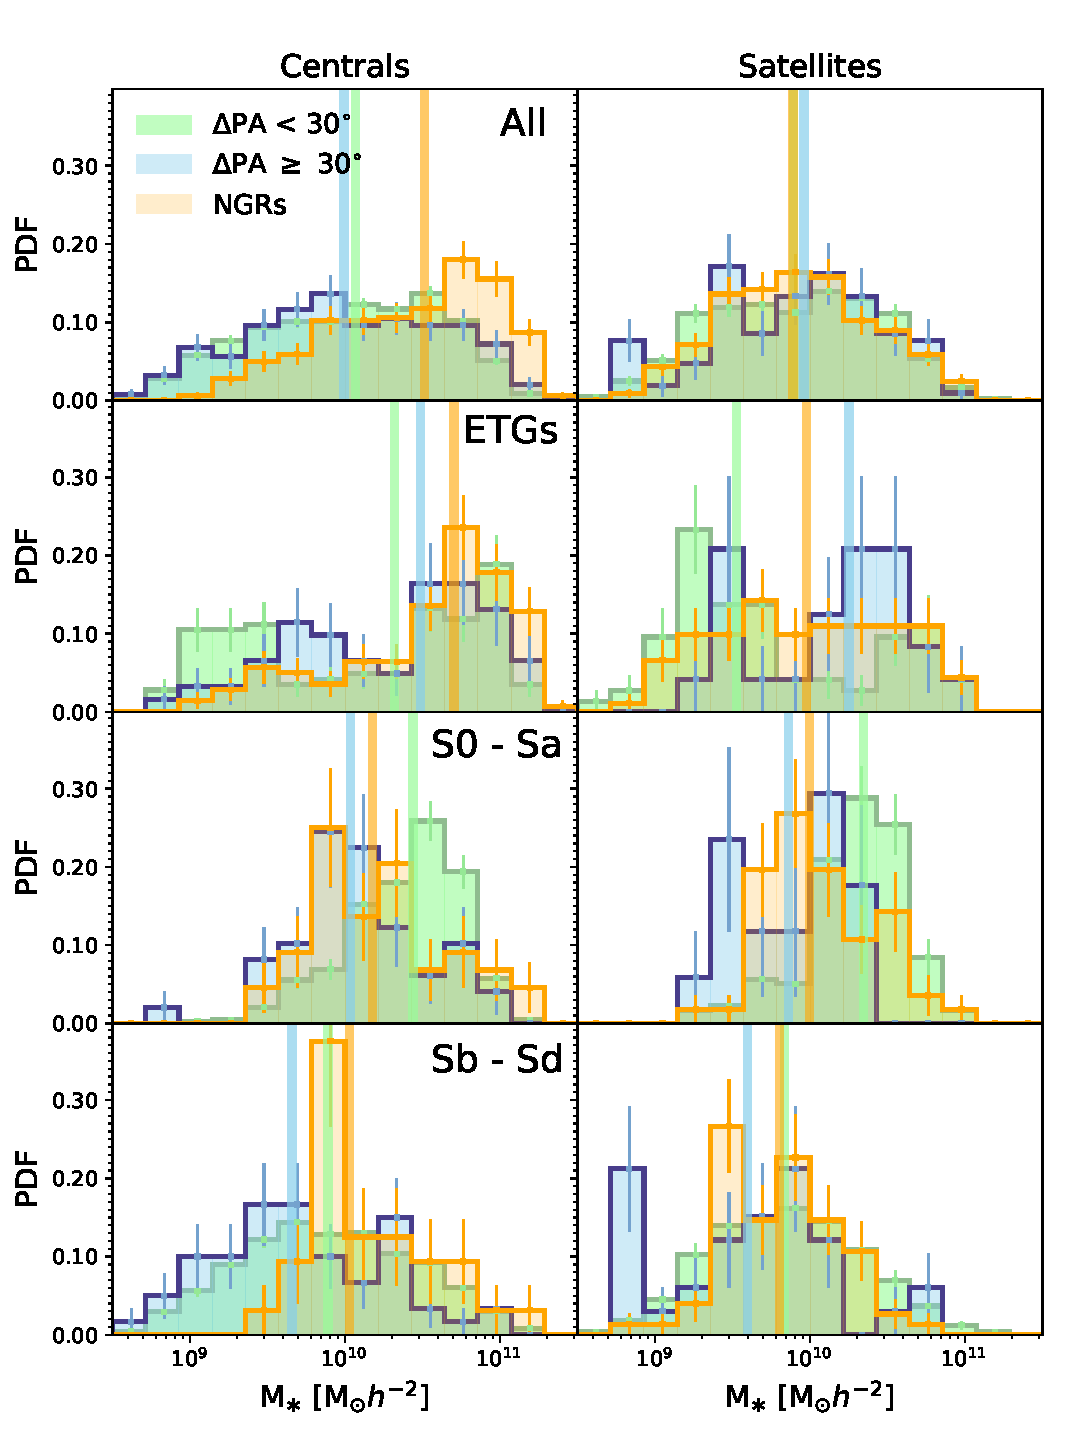
\includegraphics[width=0.85\linewidth]{misalignment_MaNGA/delPA_stelM_morph_lim_nsa.pdf}
    \caption{Same as Figure \ref{fig:morph_stelM}, however split by group membership into centrals (left) and satellites (right). Additionally the distributions for the overall central and satellite populations is shown in the top row. We see that for ETGs there is a strong difference in mass between aligned and misaligned satellites. This trend is reversed for S0/Sa and Sb/Sd satellites. These trends are also seen for centrals, however, typically to a lesser degree.}
    \label{fig:group_morph_stelM}
\end{figure*}

\section{Summary} \label{sec:summary_manga}
In this chapter, we introduce a catalogue of $\sim$4500 galaxies from the MaNGA survey in order to establish the
prevalence of misalignment as a function of optical morphology. We also relate the typical stellar angular momentum and gas content of kinematically misaligned galaxies relative to the aligned. Our conclusions are as follows:

\begin{enumerate}
    \item The prevalence of kinematic misalignment (i.e. where rotational axes of stars and gas are offset by $> 30^{\circ}$) is strongly morphological dependent with ETGs having $\sim$28\% exhibiting misalignment which decreases to $\sim$5\% for Sb-Sds.
    
    \item For all morphologies this misalignment is related to a lowered stellar angular momentum and also a lowered gas mass. We note that misaligned galaxies have similar stellar angular momentum to those do not have coherently rotating gas (those with large gas depletion fall into this category). This could be indicative that galaxies without coherent gas rotation and kinematically misaligned galaxies are different timesteps in the same evolutionary sequence. As noted in simulations \citep[][]{vdvoort2015, starkenburg+19}, a key component in decoupling star-gas rotation is a significant gas loss followed by accretion of new gas with misaligned angular momentum. In this scenario, NGRs could represent an earlier timestamp before a future re-accretion of gas. This would indicate that the stellar angular momentum is disrupted prior to accretion of new material. 
    
    \item We find that the misalignment fraction is also dependent on group membership. For ETGs and S0-Sas, central galaxies are more likely to exhibit misalignment than satellites. For Sb-Sds this trend reverses.
    
    \item We find that counter-rotation (i.e. rotational axes of stars and gas are offset by $> 150^{\circ}$) is a stable state for galaxies of all morphologies shown by a boost in the PDF (Figure \ref{fig:morph_PA}). Similar to the total misaligned population, counter-rotators have distinctly lower angular momentum than their aligned counterparts. 

\end{enumerate}

In the following chapter, we investigate whether hydrodynamical simulations can reproduce these observed trends and what typical timescales are associated with angular momentum and gas loss.